\section{Backhual Algorithm and Evaluation}
\label{sec:whitemesh}

% Organization of the Sec
In this section, we study the channel assignment problem jointly when using WiFi and white space 
bands in concert across the backhual tier of a wireless mesh network. We then present our linear programming model and 
heuristic-based measurement-driven algorithm to address the problem. 
 
\subsection{Linear Programming Formulation}
\label{subsec:linearopt}

The function of the backhual tier is to wirelessly provide end to end traffic to and from the user and Internet.
% Metrics
In practice, the traffic demand of the users obeys a Poisson process~\cite{saaty1961elements}. 
Most of the carriers charge users based on the traffic being tranferred oner the Internet. 
The traffic demand of the users delivered to or from the Internet are noted as the total traffic served. 
In particular the total traffic served $X$, is represented as:
\begin{equation}
\label{eq:goodput}
X=\sum_{w \in W, v \in V}T(w,v)
\end{equation}
$T(w,v)$ nodes all delivered traffic between access point $v \in V$ and gateway node $w \in W$.

%To clarify the problem and approach the optimization solution of the problem, 
Here, we present a linear programming formulation to approach the optimal channel assignment in along the backhaul 
tier of a WhiteMesh network. 
We leverage the nodes into consider the set of available access points ($V$) which aggregate the traffic from the users, 
and gateways ($W$) as ingress points to the Internet. The available frequency bands ($B$) are pre-known 
as an input. The conflict graph $I$ is given as parameters. 
$\delta_b$ is the achieved channel capacity estimated from the  activity level measurements 
introduced in Section.~\ref{sec:measurements}.


\noindent
{\bf Sets:}
\begin{tabular}{ll}
$V$ & set of nodes \\
$B$ & set of bands \\
\end{tabular}

\noindent
{\bf Parameters:}\\
\\
%\vspace{0.1in}
%\begin{tabular}{lll}
\begin{tabular}{llp{3.4cm}}
%\hline
$\delta^b$ & $b \in B$ & Achieved capacity of band $b$ in target area\\
%\begin{tabular}{llp{2.8cm}}
$I_{ij,lm}^b$ & $(i,j,l,m) \in V, b\in B $ & Protocol Interference of link $(i,j)$ on band $b$ brought by link $(l,m)$\\
%\hline
%\end{tabular}\\
%\begin{tabular}{llp{2.8cm}}
$W_i$ & $i \in V\ binary$ & Gateway marked with access point set\\
%\hline
%\end{tabular}\\
%\begin{tabular}{llp{2.8cm}}
$D_{d}$ & $i \in V\ $ & Downlink demand of node i\\
%\hline
%\end{tabular}\\
%\begin{tabular}{llp{2.8cm}}
$D_{u}$ & $i \in V\ $ & Uplink demand of node i\\
%\hline
\end{tabular}

The variable time share $\alpha_{i,j}^b$ represents the assigned percentage of a single link transmitting time  
for link $i,j$ between node $i$ and node $j$ in band $b$. 
The two variables, $uy_{i,j,k}^{b}$ and $dy_{i,j,k}^{b}$ are defined as uplink and downlink flows:

\noindent
%\vspace{2pt}
{\bf Variables:}\\
\\
%\vspace{1pt}
\begin{tabular}{llp{3cm}}
$0\le \alpha_{ij}^b \le 1$  & $b\in B, (i,j) \in N$ & 
Time share of link $(i,j)$ on band $b$\\ 
$0\le uy_{i,j,k}^b$ & $(i,j,k) \in V, b \in B$ & 
Uplink flow of node $k$ on link $(i,j)$ at band $b$ \\ 
$0\le dy_{i,j,k}^b$ & $(i,j,k) \in N, b \in B$ & 
Downlink flow of node $k$ on link $(i,j)$ at band $b$ \\ 
\end{tabular}
\vspace{1pt}

% FIXME talk about NT calculation
The objective is to maximize the total traffic served ($X$) of all the gateways, $X$ is defined in Eq.~\ref{eq:goodput}.
It is represented with the variables:

\noindent
{\bf Objective:}
\begin{align}
& Max \sum_i\sum_j\sum_k\sum_b(uy_{i,j,k}^b+dy_{j,i,k}^b) \;\ When \; w_j=1 
%& Max \sum_i\sum_j\sum_b(\frac{1}{\sum_{l,m}\alpha_{i,j}^b\times I_{ij,lm}})
\end{align}

In this LP formulation, the constraints are presented as connectivity, uplink, and downlink sections here:  

\noindent
%{\bf Constraints:}
{\bf Connectivity Constraints:}
\begin{align}
\label{opt:1}
& \alpha_{i,j}^b + \alpha_{j,i}^b + \sum_l\sum_m(\alpha_{l,m}^b \cdot I_{ij,lm}^b) \leq \delta^b, i\neq j \\
\label{opt:2}
& \sum_i uy_{i,j,k}^b + \sum_i dy_{i,j,k}^b \leq \delta^b \cdot \alpha_{j,k}^b 
\end{align}
\noindent
{\bf Uplink Constraints:} 
\begin{align}
\label{opt:3}
& \sum_k \sum_b uy_{i,k,i}^b \leq D_{ui}  \; ; w_k=0, i \neq k \\
\label{opt:4}
& uy_{i,j,k}^b \cdot w_k = 0 \\
%\label{opt:5}
%& \sum_i\sum_b uy_{i,j,k}^b - \sum_m\sum_b uy_{j,m,k}^b = 0 \; when \; w_k=0, i\neq k\\
\label{opt:6}
& \sum_{i\neq j}\sum_b uy_{i,j,k}^b = \sum_{m\neq j} \sum_b uy_{j,m,k}^b \; ;w_j = 0\\
\label{opt:7}
& uy_{i,j,i}^b=0 
\end{align}
\noindent
{\bf Downlink Constraints:} 
\begin{align}
{\bf}
\label{opt:8}
& \sum_k \sum_b dy_{i,k,i}^b \leq D_{di} \; \; ; w_k=0 \\
\label{opt:9}
& dy_{i,j,k}^b =0  \; ;w_k=1 \\
%\label{opt:10}
%& \sum_j\sum_b dy_{i,j,k}^b - \sum_m\sum_b dy_{i,k,m}^b \geq , i \neq k \\
\label{opt:11}
& \sum_{i\neq j} \sum_b dy_{i,j,k}^b = \sum_{m \neq j} \sum_b dy_{j,m,k}^b   \; ; w_j=0, i \neq k \\
\label{opt:12}
& dy_{i,i,j}^b=0
\end{align}

In these constraints, (\ref{opt:1}) represents the total time assigned for the incoming flows, outgoing flows, 
and the interfering time which should all be less than 1. Constraint (\ref{opt:2}) represents that the incoming and 
outgoing wireless traffic are less than the capacity assigned for link $i,j$. Uplink constraints 
(\ref{opt:3}) and (\ref{opt:4}) represent that the total traffic flow on link $i,j$ from $i$ is less than 
the demand of node $i$. Constraints (\ref{opt:6}) and (\ref{opt:7}) restricts the sum of incoming data 
flows for a given access point $k$ equal to the total outgoing flows from the node. Downlink constraints 
(\ref{opt:8}) and (\ref{opt:9}) represent similar restrictions as (\ref{opt:3}) and (\ref{opt:4}), but 
in the downlink direction. Similarly, constraints (\ref{opt:11}) and (\ref{opt:12}) are downlink versions of 
(\ref{opt:6}) and (\ref{opt:7}).
Since linear programming models for multiple channels has been proved to be NP-hard~\cite{yuan2006cross},
in this work, we choose small set of cases to achieve the optimal solution.



% PEN part 
%% Talk about the network efficiency for multiband multihop mixed hop

In ~\emph{Multiband Multiradio Network}, 
a multihop path could have higher frequency band combination with less interference range or a set of lower frequency band with less hop count.
A key issue of multihop path in such network is to answer which combination is better.
We focus our work on ~\emph{Channel Assignment} dealing with more interference factors rather than routing protocol which would be more concern on delay. Other architecture also has such problem such as wireless sensor network.

To discuss this problem, we pick up a multihop path from mesh network and analyze its performance with worst case hypothesis. In mesh network, such a path would have a bottle neck in the link closet to gateway.
When a mesh network was built with gateway placement, constructor should considered load-aware demand of mesh nodes and mesh node population. 
Generally the nodes close to gateway should have more traffic demand and gateway itself should have the most connectivity population. 
We treat each node equally binding with fairness, otherwise mesh nodes close to gateway could be served more traffic and show a high goodput of the network.
For analyze, we assume all the node in the path equally share the time of the link next to a gateway. It is also the worst case for getting a larger goodput.


First, we introduce the ~\emph{Intra-Path} traffic. When we have a multihop path, in worst case all the nodes on the path have only one $h$ hop path arrived at a gateway node. The path is made of links from one node to another.
Each node has traffic $T$, nomatter uplink or downlink since both of them occupy link capacity in the same way. And the total traffic on the path $\sum T$ is less than the bottle neck link capacity $C$. 

We define the minimum transmission rate on a path as ~\emph{Network Efficiency}. 
With the fairness restriction, the last node in the path has the minimum transmission rate.
Then the acitve time in a time unit of each link can be represented as $1,\frac{h-1}{h},\frac{h-2}{h}\cdots \frac{1}{h}$. 
The unit time of each link in the path is counted as total cost time of network.
%\begin{equation}
%\label{eq:intrapath}
%\begin{split}
%E_{Intra-Path}=\frac{Path\ Active\ Time}{Network\ Time}\\
%E_{Intra-Path}=\frac{1}{2}+\frac{1}{2\cdot h}
%\end{split}
%\end{equation}


%As hop count increase, the ~\emph{Intra-Path} will decrease till the lower bound $\frac{1}{2}$. With routing protocol which is out of this work, the delay increase too.
Without considering ~\emph{Inter-Path} interference which represent interference with links out of the path, 
an intuition of using lower band is to reduce the hop count
 to increase the minimum time utility rate which is the active time of the last link over the total active time of the path. 
However, at the same time, the interference range increase too. An example shown in ~\ref{fig:networkefficiency}, 
the picture shows links in different bands, let's say 2.4GHz and 900MHz, as a sketch map, does not represent the real distance.
Node $A,C$ could be connected through two 2.4GHz links or a single 900MHz link; with 2.4GHz links, only link $D,E$ will be interferenced; however, with 900MHz $A,C$ link, link $F,G;M,L;K,J$ will be interferenced. 


\begin{figure}
%\vspace{-0.0in}
\centering
\includegraphics[width=74mm]{figures/networkefficiency}
\vspace{-0.1in}
\caption{Path Network Efficiency Introduction, Solid Wire notes 2.4GHz link, Dashed line notes 900MHz}
\label{fig:networkefficiency}
%\vspace{-0.0in}
a\end{figure}

To quantization this ~\emph{Inter-Path Interference}, 
the unit time of these links are counted as ~\emph{Network Time}. 
When a $h$ hop path transmitting traffic $T$ for the destination node, it stops activity on a number of links in the same band. 
In a multihop path, when the traffic arrived at the last destination node, all the previous links are serving for these traffic.
The active time on a single link can be noted as 
$\frac{T}{c_h}$. We keep in the worst case when the last node in the path got traffic $T$, the other node also be served traffic $T$.
With interference counts $I_h$ from the conflict matrix:
the ~\emph{Network Time} counted as 
$\frac{hT}{c_1}\cdot I_1 + \frac{(h-1)T}{c_2}\cdot I_2 \cdots \frac{T}{c_h}\cdot I_h$, the ~\emph{Path Efficiency over Network} is defined the traffic over the ~\emph{Network Time} and could be represented as:



\begin{equation}
\label{eq:originpen}
E_{PEN}=\frac{T}{\sum_{i \leq h}\frac{i\cdot T}{c_h}\cdot I_i }
\end{equation}

With protocol model, if link exist, then they have the same capacity $c_1=c_2 \cdots =c_h=c$. 
To avoid $0$ value in the denominator, we add a $1$ to adjust the denominator which does not change the parameter characteristics. 
The \emph{Path Efficiency over Network}could be represented as:


\begin{equation}
\label{eq:pen}
E_{PEN}=(\frac{c}{1+\sum_{i \leq h} i\cdot I_i}
\end{equation}
 

The meaning of the ~\emph{Network Efficiency} is that in a unit time, the traffic could be loaded by this path. In multichannel scenario, all the channel will have the same communication range, this parameter equals to the conflic graph in many multichannel works which try to minimize the interference~\cite{jain2005impact}. Since we count only one channel not all possible links, it also could be seen as an extention of a single link ~\emph{Link Load} defined in ~\cite{raniwala2004centralized}.

The ~\emph{Path Efficiency over Network} connect hop counts and interference. 
Then we discuss when a lower ~\emph{White Space Band} is better to be used in a path.
In a path, we use an average interference count $\bar{I}$ replace each interference count with assumption the links in the path all in one higher freq band. Then a ~\emph{White Space Band} is used to replace two links in the path as a single link with interference count $X$ represent one of the factor $i\cdot I_i$. The problem could be formulated as:

 
\begin{equation}
\label{eq:benefit}
\frac{c}{1+\frac{h(h-1)}{2}\cdot \bar{I}+X} \geq \frac{c}{1+\frac{h(h+1)}{2}\cdot \bar{I}}
\end{equation}

From the inequation, when $X \leq 2\cdot h\bar{I}$ a lower band could be better. $X$ is also a function of hop order in the path, generally the path order lower, the threshold would be more strict; otherwise it could be loose. It matches the intuition the hop order is small, it close to the gateway, it should be more crowd for this link.
It helps to tell the ranking of set of links and a path where we can start to resolve channel assignment problem.









\subsection{Path Interference Induced on the Network}
\label{subsec:PEN}

In WhiteMesh networks, it is possible that multihop paths are intermixed with WiFi bands for more spatial reuse 
and white space bands with hop count reduction. We analyze the band choices reducing the number of hops along 
a path and the aggregate level of interference on that hop-by-hop path choice has on the network (i.e., Path 
Interference induced on the Network).

Mesh nodes closer to the gateway generally achieve greater levels of throughput at sufficient-high 
offered loads. To combat the resulting starvation effects for downstream nodes, we treat each flow with equal priority in the network 
when assigning channels. In the worst case, all nodes along a particular path have equal time shares for 
contending links (i.e., intra-path interference). We begin the channel assignment assuming that $h$ mesh 
nodes are demanding traffic from each hop of an $h$-hop path to the gateway. If each link along the path 
uses orthogonal channels, then each link could be active simultaneously, otherwise they will compete with 
each other. We note each node along the path had traffic demand $T_d$. The bottleneck link 
along the path would be the one closest to the gateway. Thus, the total traffic along the 
path $h \cdot T_d$ must be less than the bottleneck link's achieved capacity $\delta$, estimated according 
to the measurements. The $h$-hop access point would achieve the minimum-served demand, which we define as the 
network efficiency. In general, the active time per link for an $h$-hop access point can be represented by 
$1,\frac{h-1}{h},\frac{h-2}{h}\cdots \frac{1}{h}$. The summation of all active times for each access point 
along the path is considered the intra-path network cost.


Using lower carrier frequencies allows a reduction in hop count and increase the network efficiency of each 
access point along the $h$-hop path by reducing the interference among the links of the path. However, a lower 
carrier frequency will induce greater interference to other paths to the gateway (i.e., inter-path interference). 
When an $h$-hop flow is transmitted to a destination node, it prevents activity on a number of links in the 
same frequency via the protocol model. The active time on a single link is noted as $\frac{T}{\gamma_h}$. 
An interfering link from the conflict matrix $F$ counts as $I_h$ per unit time and contributes to the network 
time cost in terms of:
$\frac{hT}{\gamma_1}\cdot I_1 + \frac{(h-1)T}{\gamma_2}\cdot I_2 \cdots \frac{T}{\gamma_h}\cdot I_h$.
Then, the traffic transmitted in a unit time of network cost for the $h$-hop node is:
\begin{equation}
\label{eq:originpen}
E_{\eta}=\frac{T}{\sum_{i \in h}\frac{(h-i+1)\cdot T}{\gamma_i}\cdot I_i }
\end{equation}
Through network efficiency, the equation simplifies to:
\begin{equation}
\label{eq:pen}
E_{\eta}=\frac{\gamma}{\sum_{i \in h} (h-i+1)\cdot I_i}
\end{equation}

Network efficiency is the amount of traffic that could be offered on a path per unit time. With 
multiple channels from the same band, $I_i$ will not change due to the common communication 
range. With multiple bands, $I_i$ depends on the band choice due to the communication range 
diversity. Network efficiency jointly considers hop count and interference in the paths. We define
the Path Interference induced on the Network (PIN) as the denominator of Eq.~\ref{eq:pen}.
The parameter represents the sum of all interfering links in the network by a given path. 

PIN is used to quantify the current state of channel for channel assignment across WiFi and 
white space bands. To determine when the lower carrier frequency will be better than two or 
more hops at a higher carrier frequency, we consider the average interference $\bar{I}$ of 
a given path at the higher frequency. The problem could be formulated as:
\begin{equation}
\label{eq:benefit}
\frac{\gamma}{\frac{h(h-1)}{2}\cdot \bar{I}+I_x} \geq \frac{\gamma}{\frac{h(h+1)}{2}\cdot \bar{I}}
\end{equation}

Here, from Eq.~\ref{eq:benefit}, when $I_x \leq 2\cdot h\bar{I}$, the performance of a 
lower-frequency link has better network efficiency than two higher-frequency hops for 
the same destination node. $I_x$ is also a parameter of hop count in Eq.~\ref{eq:pen}. 
When the hop count is lower which closer to the gateway node, the threshold would be 
more strict since the interference would have a greater effect on the performance.


\subsection{Band-based Path Selection (BPS) Algorithm}
\label{subsec:BPS}

\begin{figure}
\vspace{-0.0in}
\centering
\includegraphics[width=74mm]{figures/interferencerange2}
\vspace{-0.1in}
\caption{Example WhiteMesh topology with different mesh-node shapes 
representing different frequency band choices per link.}
\label{fig:interferencerange}
\vspace{-0.1in}
\end{figure}

% Intra network interference
Consider the following motivation example in Fig.~\ref{fig:interferencerange}, the access point $A$ could connect to access point $C$ 
relayed by node $B$ with 2.4 GHz, or directly connect to $C$ at 450 MHz. If 2.4 GHz were 
chosen, link $D,E$ is able to reuse 2.4 GHz when they are out of the interference range. 
However, along the backhual tier, if link $A,C$ used 450 MHz, a lower hop count would 
result for the path, yet lower levels of spatial reuse also result (e.g., for link $D,E$). 
While the issues of propagation, interference, and spatial reuse are simple to understand, 
the joint use of white space and WiFi bands to form optimal WhiteMesh topologies is 
challenging since the optimization is based on the knowledge of prior channel assignment 
which is not available before the work has been done.

Thus, in the backhaul tier, we formulate the problem with a graph-based model. A connectivity graph $C$ is 
formed for each band in $B$ such that $C=(V,L,B)$. If the received signal for a given band is 
above an interference-range threshold, then contention occurs between nodes. We extend the conflict 
matrix in~\cite{tang2005interference} related to the interference per band according to 
$F=(E_{i,j},I_{Set},B)$, where $E_{i,j}$ represents the link and $I_{Set}$ includes all the links 
are physically inside the interference range $D_r$ when operating on each band $b \in B$.

Therefore, the problem we model is: choose the connectivity graph $C'$ which maximizes the total traffic served 
from the access tier. A key challenge is that selecting the optimal channels from the 
set $B$ leads to a conflict graph $F$ which cannot be known {\it a priori}. 

%Previous works have proposed 
%several coloring, cluster-independent set, mixed linear integer methodology for a single band $b$ 
%~\cite{peng2012efficient,tang2005interference,doraghinejad2014channel}. 
%However, these works fails to address a reduction in hop count or an increase in spatial reuse and 
%channel occupancy for a set of diverse bands $B$.

\begin{algorithm}[t]
    \small
\caption{Band-based Path Selection (BPS)}
\begin{algorithmic}[1]
\label{algorithms:bps}
\REQUIRE  ~~\\
	$M$: Set of access points\\
	$G$: Set of gateway nodes\\
	$C$: Communication graph of potential links among all nodes\\
	$I$: Interference matrix of all potential links \\
	$B$: Available frequency bands \\
	$\delta$: Measurements based Channel Capacity
\ENSURE ~~\\    
$CA$: Channel Assignment of the Network\\
\STATE Rank access points in Set $M$ according to physical distance from gateway nodes $G$
\STATE Initialize $S_{curr}=G$, $N_{srv}=\emptyset$, $N_{unsrv}=M$,$I_{active}=\emptyset$
\WHILE {$N_{srv}=!M$}
\STATE Select node with largest distance to gateway
\STATE Find the adjacency matrix across band combinations $A_c$
\FORALL{$A_{i}\in A_c$}
\STATE Find the shortest path $SP_i$ in mixed adjacency matrix A 
\FORALL{Link $l \in SP_i$, ordered from gateway to access point}
\STATE Find the least interfering path with measured $\delta \times E_n$
\STATE If equally-interfering links, choose higher frequency
\STATE Calculate the path interference of $SP_i$
\ENDFOR
\STATE Store the shortest path $SP_i$ as $SP$
\ENDFOR
\STATE Assign the path in the network\\
		\STATE Update $N_{srv},N_{unsrv}$
		\STATE Update $I_{active}$ from $I$
\ENDWHILE \\
Update $CA$ as the locally-optimal solution\\
\end{algorithmic}
\end{algorithm}


We design a Band-based Path Selection (BPS) algorithm shown in Alg.~\ref{algorithms:bps}. 
The algorithm first chooses the access point that has the largest physical distance from the 
gateway nodes in the network to most greatly reduce the total time cost of the network. 
When a path is constructed for the access point with the greatest distance, all 
subsequent access points along the path are also connected to the gateway. 
In large-scale mesh networks, the complexity makes it impractical to traverse all the 
paths with different combination of bands from an access point to any gateway node. It has been 
proved as an NP-hard problem. However, based on the discussion in Section.~\ref{subsec:PEN}, 
if two paths have the same number of used bands along those paths, then the path with the 
least hops is likely to have the greatest performance and is chosen. Similarly, if two path 
have the same path interference, we choose the path which has higher-frequency links to keep 
the potential improvement of spatial reuse. Thus, the next step of the algorithm is to find 
the shortest path across band combinations.

In the algorithm, compared to the number of access points, the amount of channels $N_B$ in
different bands is small. The time complexity of calculating the combination is $O(2^{N_B})$. 
Finding the shortest path in Dijkstra algorithm will cost $O(N_E^2)$~\cite{golden1976shortest}, 
where as $N_E$ is the set of possible links in the network. As a result, the total complexity 
would be $O(N_E^2\cdot 2^{N_B})$. 
The algorithm will compare the PIN of the candidate paths and select the path with the 
least interference channel induced on the network for the source access point.
The algorithm updates the channel assignment of the network after the path is chosen.
Then, the set of served nodes, activated links, and radio information are updated. 
The process will repeat iteratively to assign channels for all the access points in the
network.

The complexity of assigning a channel for an access point is $O(N_E^2\cdot2^{N_B})$ 
if all the nodes are connected to gateway nodes ($N_E={n \choose 2}$ which is $O(N_V^2)$). 
The complexity of assigning an access point is $O(N_V^4\cdot2^{N_B})$.
To assign {\it all} the access points in the network, the complexity would be 
$O(N_V^5\cdot2^{N_B})$. The complexity is polynomial time of the number of traffic 
demands points (mesh group) for a wireless network assignment.


\subsection{Experimental Evaluation Setup}
\label{subsec:design}
% Simulation Setup
WhiteMesh networks have the diversity in propagation from the lowest white space channels 
(tens to hundreds of MHz) to the highest WiFi channels (multiple GHz). We consider a wide range 
of propagation characteristics from four different frequency bands to set up the experimental 
evaluation. We use 450 MHz and 800 MHz of white space bands and 2.4 GHz and 5.2 GHz of WiFi bands
data from the spectral analysis in Section.~\ref{sec:measurements}.

% Network Setup
According to the population density for a given deployment location, we consider the spectral activity observed for 
the population density from our in-field measurement.
We input the measurements to both the LP and heuristic-based algorithm to compare 
the performance in various scenarios. The communication threshold is set as -100 dBm. The 
communication range is normalized with the highest frequency of 5.2 GHz. Then, the communication 
range of 450 MHz, 800 MHz, 2.4 GHz, and 5.2 GHz would be normalized to 12.8, 6.2, 2.4, and 1, 
respectively in the Friis model (as Eq.~\ref{eq:friis}). 
The interference range is set to twice that of the communication range~\cite{raniwala2005architecture}. 
We deploy static wireless mesh networks of $n$ access points along a regular grid with a normalized 
distance of 0.8 between rectangular edges. The gateways are chosen through a typical cell hexagon 
deployment method based on 2.4 GHz~\cite{meguerdichian2001exposure}. Unless otherwise specified 
in the analysis, all four bands are used in the WhiteMesh topology studied. For practical application 
scenarios, more channels could be considered by BPS algorithm.


% Traffic generation
The traffic demand aggregated by an access point is independent to others and obeys a Poison distribution
per unit time. 
In the simulation, we generate an equal number of access points (including both gateway nodes and 
access points) Poison random numbers with a mean of $\lambda$. 
Then, we assign as the traffic demand for each access points in the 
target area.
% total traffic served calculation
As mentioned previously, the achieved wireless capacity of gateway nodes has been shown to be the 
bottleneck in mesh networks~\cite{robinson2010deploying}. Moreover, the amount of total traffic served is affected 
by access point placement, gateway placement, routing, and channel assignment. For the purposes 
of our analysis, we specifically calculate the total traffic served through a greedy strategy. 
We study the channel assignment process under a tree-based structure. 
To maximize the total traffic served, we start to serve the traffic demand from the gateway nodes. 
Mesh nodes that have a lower hop count path to the gateways are served first. 
When access points have the same hop count, the least interfering access points are chosen to 
reduce the cost for the whole network. When the paths have the same level of interference, the ties 
are broken by the nodes order.
The process repeats until no remaining traffic demand of users 
is unserved or no remaining channel capacity exists on any path.

We investigate the impacts of network size, band availablity, and channel occupancy on WhiteMesh networks 
in the simulations.
We assume 30\% of the residents will use the service. An individual user would have a 2 MBps 
traffic demand on average. Each radio has 600 MBps capacity as previous configuration.
We assign the traffic demand to users under the same Poison setting and 
run the analysis of each case 20 times. To approach the total traffic served upper bound, we relax our LP 
model to only keep the link capacity constraints, given the traffic demand of the access points as a 
parameter to achieve the maximum throughput at the gateways. We further compare BPS with the 
{\it (i)} Common Channel Assignment (CCA) from~\cite{draves2004routing},
and {\it (ii)} Breath First Search Channel Assignment (BFS-CA) from~\cite{tang2005interference}
under the same setup.
The CCA~\cite{draves2004routing} algorithm assigns a common channel for two nodes when both of them 
share available radios working on the same channel. In the BFS-CA~\cite{tang2005interference} algorithm, 
a node will search all the available single-hop connections and then choose the one that has the largest 
free capacity for a new assignment. 
These two methods are designed for multi-channel scenarios 
where each channel has tha same propagation characteristics and spectral activity 
level of the algorithms.



\subsection{Experimental Analysis of WhiteMesh Backhaul}
\label{subsec:wmanalysis}

\subsubsection{Network Size \& Bands Effect}

% ILP bound
Typically, the traffic patterns of access points from users are diverse with
the download direction dominating the total traffic demand (e.g., consider
service agreements for cellular data or Internet connectivity). 
Hence, to simplify the analysis and scale the LP Bound to larger network 
sizes, we only consider the download traffic in the simulations.

We investigate the network size impact on WhiteMesh networks. 
The number of access points is varied from $16$ to $64$ in the aforementioned 
regular grid. 
The gateways through the hexagonal gateway node deployment with the network 
size.
Fig.~\ref{fig:varysize} shows the results of the total traffic served 
when the population distribution is 500 $ppl/km^2$ 
for the LP formulation and the heuristic-based algorithms: 
{\it (i)} Common Channel Assignment (CCA) from~\cite{draves2004routing},
{\it (ii)} Breadth First Search Channel Assignment (BFS-CA) from~\cite{ramachandran2006interference},
AND {\it (iii)} our algorithm BPS (Section~\ref{subsec:BPS}).


\begin{figure}[t]
\centering
\subfigure[Average Population Distribution = 500 $ppl/km^2$]{
\label{fig:varysize}
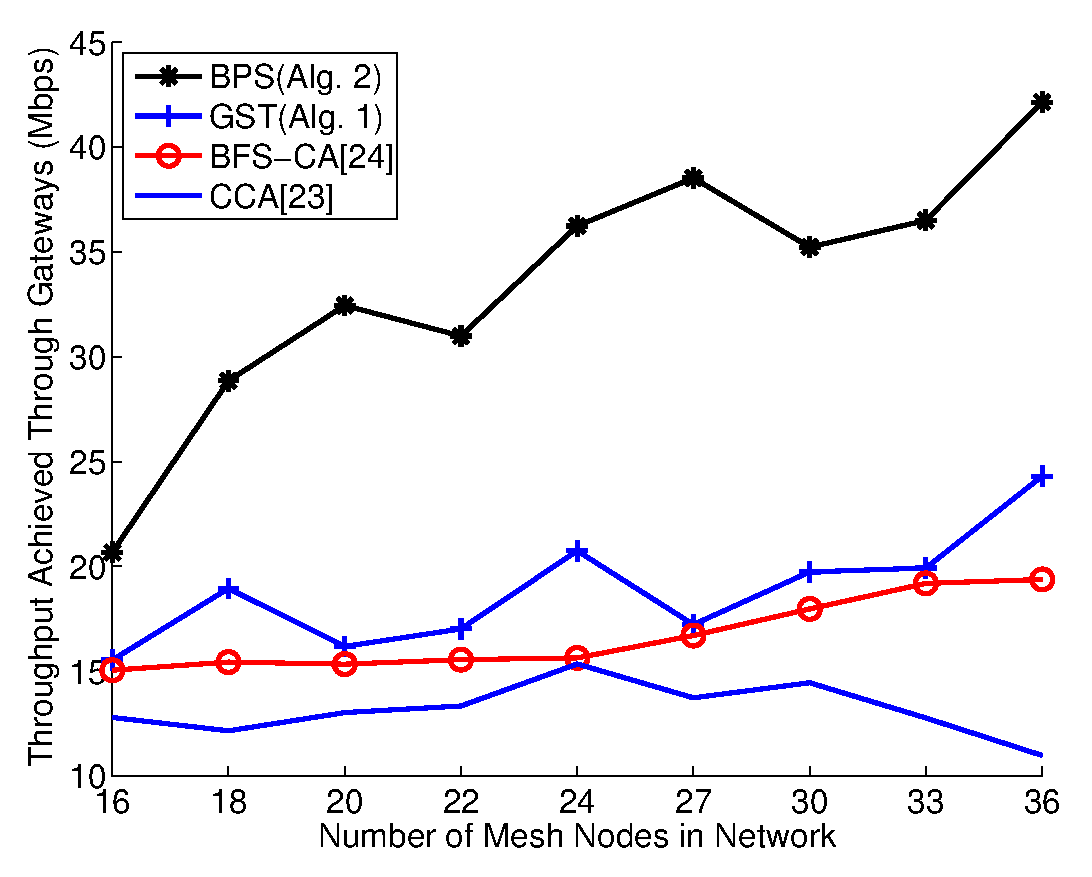
\includegraphics[width=1.6in]{figures/varysize}}
\subfigure[Varying Load, 49-Nodes Regular Grid]{
\label{fig:maxtpt}
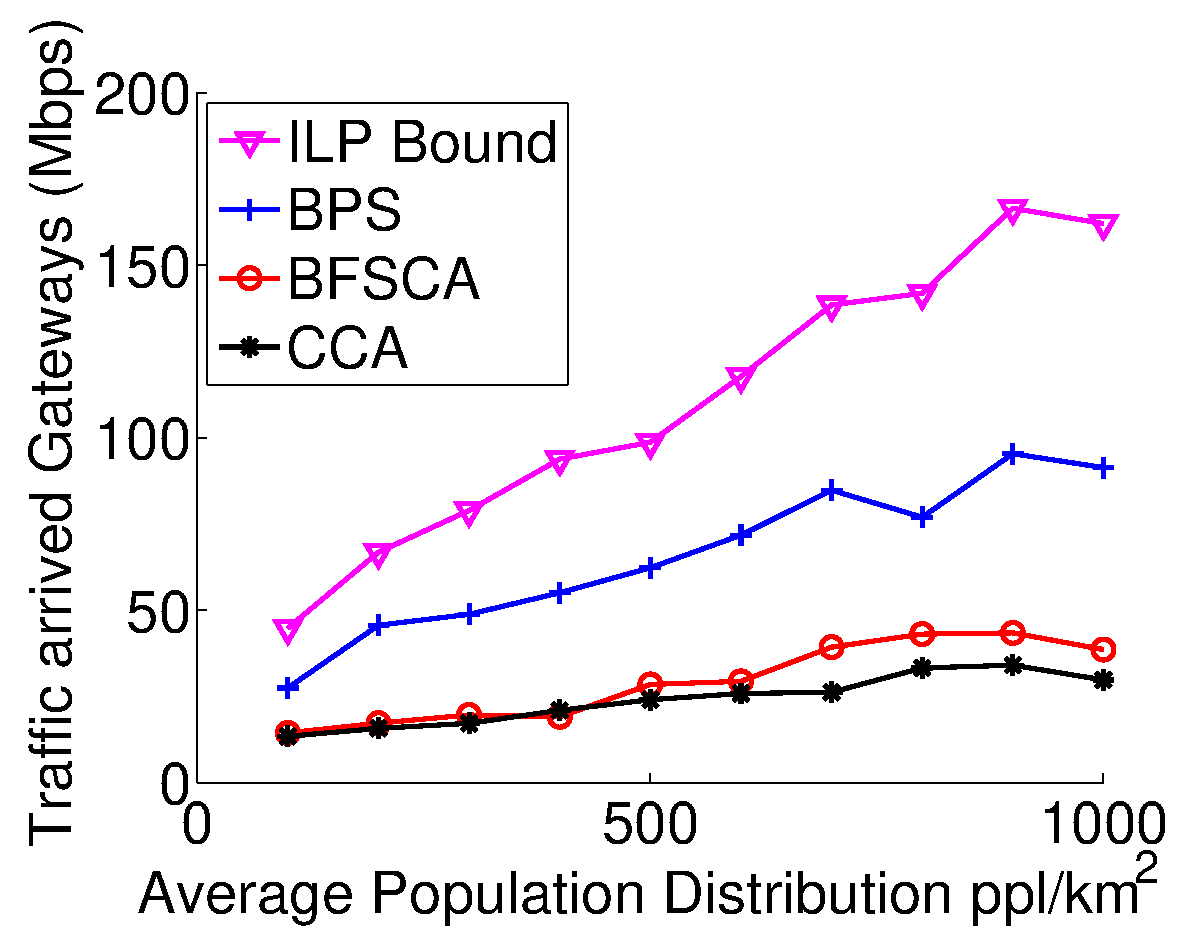
\includegraphics[width=1.6in]{figures/maxtpt.eps}}
\hfill
\caption{Performance in terms of total traffic served for various offered loads, network sizes, and configurations of WiFi or white space (WS) channels.}
\label{fig:all3figs}
\vspace{-0.3in}
\end{figure}
%\end{figure*}

In Fig.~\ref{fig:varysize}, we observe the total traffic served increases with the network size. 
The multiband wireless network has a similar communication and interference performance with 
the multi-channel wireless network with a small network size for all algorithms. 
However, as the network size or population increases, the performance diverges between BPS and 
CCA/BFS-CA.
The nodes of a small network are located in a single interference space of all the bands.
The communication range variation of the bands impact on the network performance when the inter-node spacing become diverse. 
The LP Bound shows the upper-bound of total traffic served increases with the network size.
The multi-channel algorithms assign channels without considering the channel capacity diversity and thepropagation 
differences per band. Hence, the performance 
is remains low across population densities. 
CCA fails to employ the communication range variation to find the most efficient multi hop paths. 
BFS-CA optimizes the first-hop connection from the gateway, but fails to deal the whole path 
from the gateway to destination node. Conversely, BPS alleviates the strain on these first-hop, 
bottleneck links, achieving average 76\% of the LP Bound. The gap of BPS to the LP is partly because 
BPS only considers a fixed multihop path to a gateway node for each access point, whereas the 
LP considers multiple paths to the gateways. For BPS and other heuristic-based algorithms, a dynamic 
assignment version could be implemented through updating the assignment as after path emerge.

\begin{table*}
\centering % centering table 
\begin{tabular}{|c|c|c|c|c|c|c|c|c|c|c|c|} % creating 12 columns 
\hline %\hline % inserting double-line 
%Bands     & \multicolumn{3}{c|}{Dallas} & \multicolumn{3}{c|}{Weatherford} & \multicolumn{3}{c|}{Millsap} \\% [0.5ex]
%\hline % inserts single-line 
% Entering 1st row 
 \multirow{2}{*}{Frequency Bands} & \multicolumn{9}{|c|}{Population Distribution $ppl/km^2$} \\
\cline{2-10}
		& 1500 & 1000 & 500 & 300 &  200 & 150 & 100 & 20 & 10 \\ % [0.5ex]
\hline % inserts single-line 
450 MHz &24.37	&25.83  &23.77	&6.05 &12.50  &14.03 & 7.00 & 0.07 & 0.02 \\      
\hline % inserts single-line                                                                                                       
800 MHz &4.40 	&16.49  &4.77	&5.22&5.07 &4.43  & 3.87 & 4.20 & 3.60 \\      
\hline % inserts single-line                                                                                                      
2.4 GHz &15.87 	&34.95  &2.60	&2.03&2.03 &2.77  & 2.07 & 1.60 & 0.80 \\      
\hline % inserts single-line                                                                                                     
5.2 GHz &19.70	&35.46  &1.53	&1.93&1.93 &1.33  & 1.27 & 2.07 & 2.10 \\      
\hline % inserts single-line 
\end{tabular}    
\caption{Activity Level under Population Distribution} % title name of the table 
\label{tab:activitymeasurement}    
\vspace{-0.3in}
\end{table*}    

% additional Simulation set up
Then we investigate a different form of scalability in our analysis.  Namely,
we increase the average population distribution from 100 to 1,000 per $km^2$, while
maintaining a 49-node regular grid topology. The achieved channel capacity is mapped 
to the spectral analysis with the closest population distribution. 
%
%measurements has the same distance to the current set up, the lower population 
%measurement will be chosen, for instance, we map $400 ppl/km^2$ to $300 ppl/km^2$ 
%measurements as shown in Table.~\ref{tab:activitymeasurement}. 
%
Fig.~\ref{fig:maxtpt} shows the correlation of the population distribution and total traffic served. 
Similar to Fig.~\ref{fig:varysize}, as shown in the figure, the wireless channel capacity of a 
gateway is saturated quickly when the algorithm fails to 
reduce the interference via resource allocation among the channels.
Also, the results show how the achieved channel capacity impacts on the performance. 
As the population density increases, the measurement-based channel capacity varies among multiple 
bands. When the population density reaches 1,000 $ppl$, the total traffic served decreases
due to the high measured activity level and the saturation of wireless channel capacity 
around the gateways. BPS 60\% achieve of the upper bound on average. 
The results shows that CCA and BFS-CA perform worse than BPS with limited recogination of 
propagation variation in the joint WiFi and white space scenarios.

\begin{table*}
\centering % centering table 
\begin{tabular}{|l|c|c|c|c|c|c|c|c|c|c|c|} % creating 12 columns 
\hline %\hline % inserting double-line 
Bands/     & WiFi    & WS      & WS \& & WS \& &  WS \& & WS \& & WS \&      &  WS \&      & Multi-WS \& & Multi-WS \& & Multi-WS \& \\% [0.5ex]
Algorithms & Only    & Only    & WiFi  & WiFi  &  WiFi  & WiFi  & Multi-WiFi &  Multi-WiFi & WiFi        & WiFi        & Multi-WiFi  \\
\hline % inserts single-line 
% Entering 1st row 
WS (MHz)   &                                                        & 450,800 & 450 &  800  &  450   & 800               & 450    & 800      & 450,800     & 450,800     & 450,800     \\
\hline
WiFi (GHz) & 2.4, 5 &                                                             & 2.4 &  2.4  &  5   & 5               & 2.4, 5& 2.4, 5        & 2.4             & 5         & 2.4, 5     \\ % [0.5ex]
\hline
\hline % inserts single-line 
CCA~\cite{draves2004routing}                & 22.4   &  13.4  & 13.2    &12.5    & 16.9       & 23.2   &  24.1  &   30.6&  25.2  &       23.9       &   30.4          \\      
\hline % inserts single-line                                                                                                       
BFS-CA~\cite{ramachandran2006interference}  & 26.3   &  15.8  & 14.9    & 19.4   & 22.7       & 28.4   &  38.9  &   33.7&  30.1  &       27.4       &       36.6      \\      
%\hline % inserts single-line                                                                                                      
%GST (Alg. 1)                                                            & 11.6  &   6.6 & 9.3    &   15.1&   15.8        &  14.4  &   16.6   &    14.1  &   18.8            &  15.0           &    25.1         \\      
\hline % inserts single-line                                                                                                     
BPS (Alg. 1)                                & 41.2   & 34.1   &  38.2  & 40.0    & 35.4       & 42.8   & 58.4   &  64.9 &  54.4  &       51.9       &       63.1      \\      
\hline % inserts single-line 
\end{tabular}    
\caption{ total traffic served (Mbps) for various combinations of WiFi and Average Population Distribution = 500 $ppl/km^2$, Network Size = 49 access points).} % title name of the table 
% NEWClaim fix
\label{tab:2channelcombination}    
\vspace{-0.4in}
\end{table*}    


WhiteMesh networks are able to deploy across a vast array of environments, from
rural to urban areas. Each of these areas will have varying amounts of user
demand traffic in proportion to the population densities. 
However, since a greater number of TV stations exist in urban areas, the available 
white space bands are often inversely related to the population density. 
To capture these varying degrees of demand 
and white space availability we consider three likely scenarios and one final 
scenario for comparison purposes: {\it (i)} two WiFi bands (2.4 and
5.2 GHz) channels with two white space channels (450 and 800 MHz), {\it (ii)} 
three channels in two WiFi bands (2.4 and 5.2 GHz) with one white space channel 
(450 MHz), {\it (iii)} Four channels in two WiFi bands (2.4 and 5.2 GHz) without 
any white space channels, and {\it (iv)} four channels in two white space bands 
(450 and 800 MHz) with no WiFi bands (for comparison).

Table~\ref{tab:2channelcombination} describes the total traffic served 
for various scenarios of WiFi and white space bands with an offered load 
of 5 Mbps as mean value of Possion process from 500 $ppl/km^2$ in a regular 49-node grid. 
We study the performance of BPS in the four aforementioned scenarios of varying 
white space availability. In the simulation, we keep total 4 channels for each
method, such as in the combination of 2.4 GHz and 5 GHz, we put 2 channels in both 
bands. In the triple bands combinations, we set each band has a channel, and put the 
other channel in the highest frequency band. (In 2.4 GHz, 5GHz, 800 MHz combination, 
we put the extra channel other than the 3 channel each band in 5 GHz). 
% Justification
In the results, we observe that the WiFi-only scenario has greater total traffic served 
than the white-space-only scenario. This is due to the lack of spatial reuse achieved 
by white spaces bands. White space has larger communication range to shorten 
the hop counts as well as has larger interference reducing the spatial reuse. 
Another reason is that the achieved channel capacity of 500 $ppl/km^2$ in white 
space bands are worse than WiFi bands. These two reasons make the performance of 
white space only worse in all channel assignment methods applied here.
Interestingly, however, the joint use of both white space and WiFi bands has 
significant gains over the single type of band scenarios with the same number of 
channels (40\% greater than WiFi and 56\% over white space, on average). 

%In 500 $ppl/km^2$ scenario, 5 GHz channel is cleaner than 450 MHz which makes 
%the combination of 2 channels in 5 GHz, 1 channel in 2.4 GHz and 800 MHz has 
%better performance than WiFi(2)+WS(2) in some cases. 


In Table ~\ref{tab:2channelcombination}, that with the same number of bands (2), 
the combination with similar propagation characters, the cleaner channels combination 
has better performance. With similar achieved channel capacity, lower frequency 
offers more option for connection path perform better in channel assignment. 
If we have one channel in a white space band and one channel in a WiFi band, then 
we could employ the advantages of both WiFi for spatial reuse and white spaces to 
reduce the hop count in channel assignment. 

\subsubsection{Access Tier Impacts on Backhaul Tier}

The density of access points increase proportional to the population 
density to offer enough access capacity for the users. 
Hence, the distance among the access points and the channel 
occupancy in backhual tier channel assignment need to be leveraged.
To investigate impacts of the spacing variation and channel occupancy in the access tier 
on the backhaul tier, we perform simulation on a 49-node regular grid WhiteMesh network as
described before. 

In Fig.~\ref{fig:actspac}, we show the impacts of channel occupancy through 
the activity level and spacing variation on wireless white space mesh network. 
In the results, all the bands have the same activity level in the 49-nodes regular 
grid with normalized multiple inter-node spacing 
from 0.2 to 2.1 as discussed in Subsection~\ref{subsec:design}. In the 3-D figure, 
as the activity level increases, the total traffic served decreases due to the reduction 
of achieved channel capacity. In the spatial dimension, when the nodes have extremely
small spacing, lacking the propagation diversity of multiple bands and spacial reuse  make the total traffic served
limited as we have analyzed in Fig~\ref{fig:varysize}. 
While as the spacing gap increases, the high frequency bands
bring higher total traffic served via more spacial reuse. 
As the spacing gap increase, the high frequencies stop communicating due to the limited 
communication range. The number of available channels reductioneleads the total traffic served 
reduce sharply as shown in the figures.

We further study the real world spacing gap variation through BPS with in-field measurements.
We map the largest population distribution in Table~\ref{tab:activitymeasurement} to 
represent the spacing as normalized distance 0.2, and the least population distribution 
as normalized distance 1.7. In a regular grid the spacing distance $D_s$, population 
distribution $P_d$ and access point capacity $M_c$ obey $P_d \cdot \frac{D_s}{2} ^2 \propto M_c$. 
We interpolate activity level for each normalized distance from 0.2 to 1.7 with gap 0.1. 
The results of the heuristic-based algorithms and the results are shown in Fig.~\ref{fig:measurespacing}.

\begin{figure}[t]
\centering
\subfigure[Uniform Activity Level VS. Space Distance]{
\label{fig:actspac}
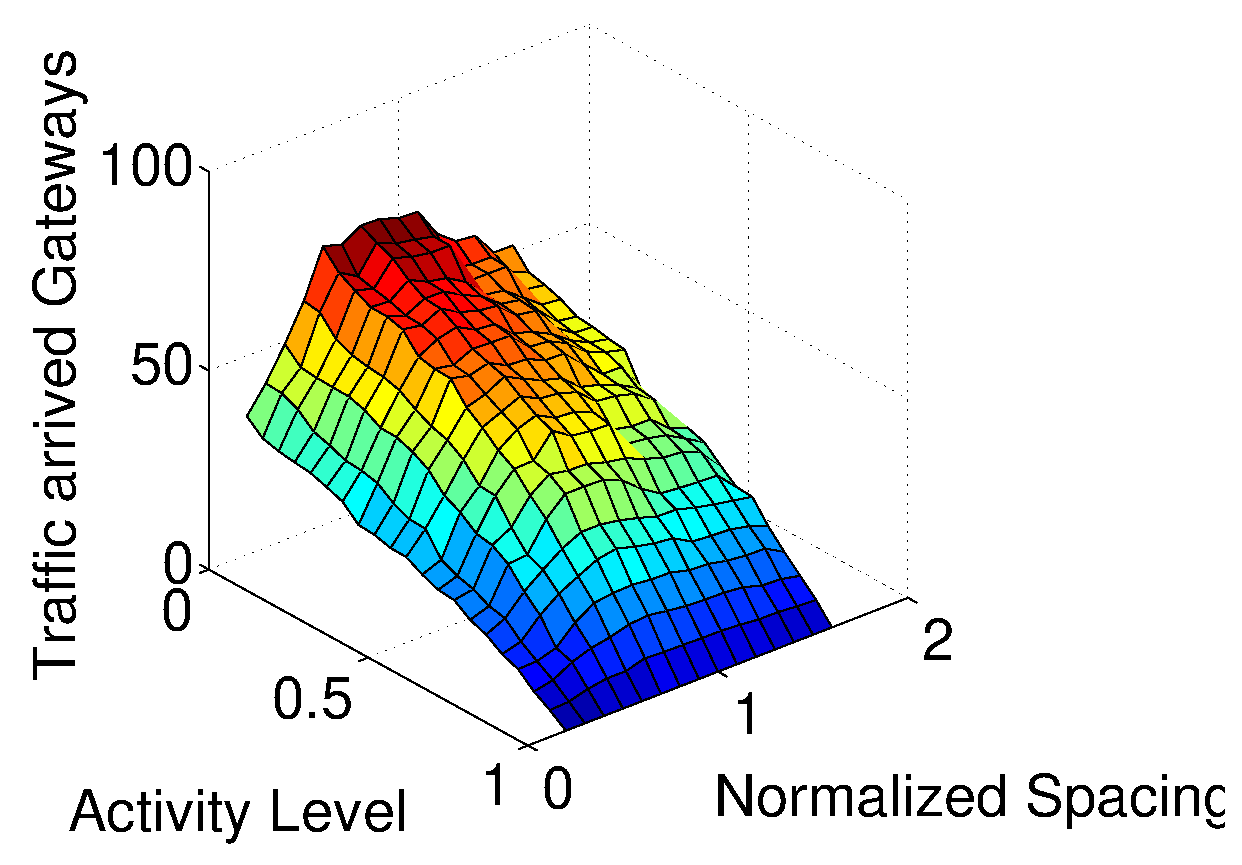
\includegraphics[width=1.6in]{figures/actspac3d}}
\subfigure[total traffic served with Activity Level \& Spacing ]{
\label{fig:measurespacing}
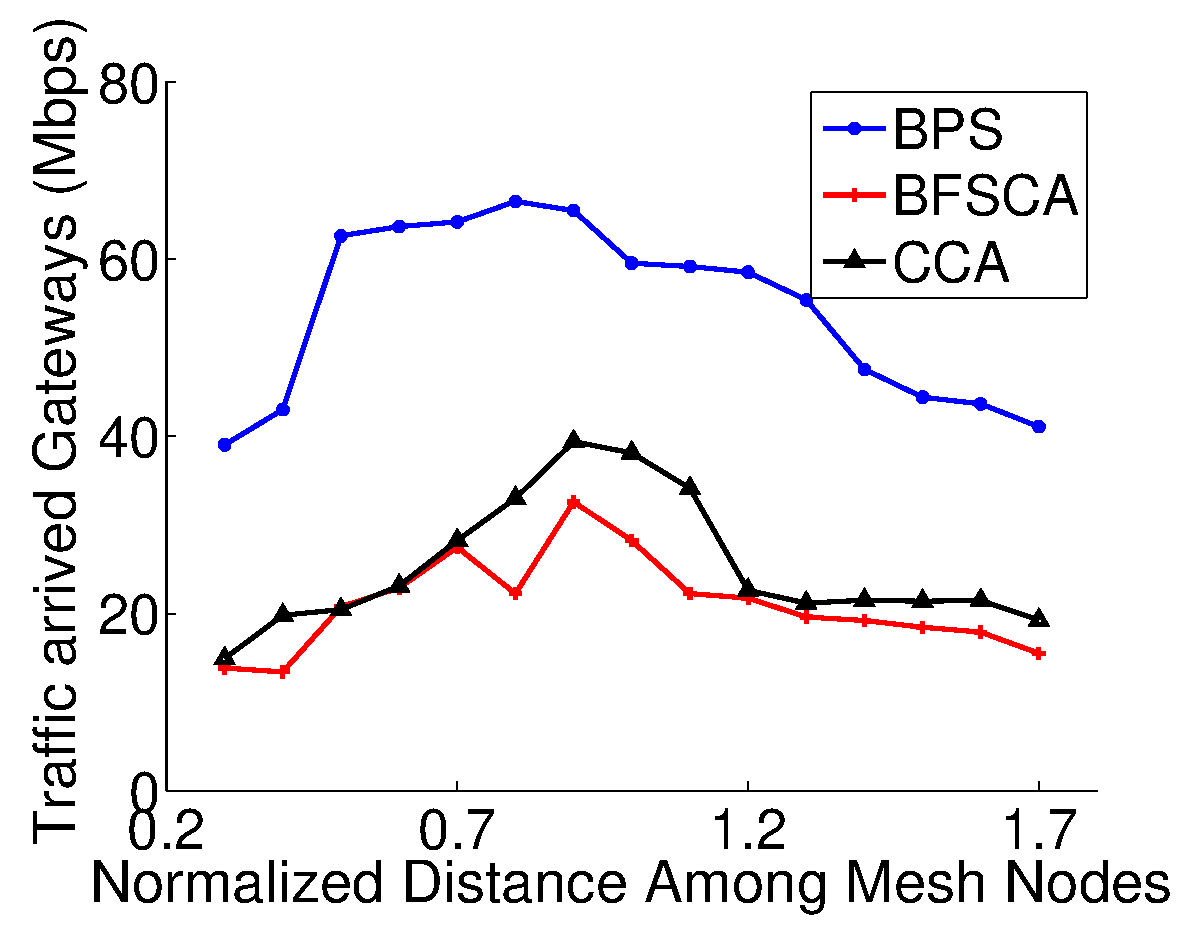
\includegraphics[width=1.6in]{figures/act_spacing}}
\hfill
\caption{Spacing Impacts on the Backhaul Tier}
\label{fig:all3figs}
\vspace{-0.3in}
\end{figure}

In Fig.~\ref{fig:measurespacing}, as the spacing increases, the WhiteMesh network 
has the best performance in all methods through spatial reuse, matching the simulation 
analysis shown in Fig.~\ref{fig:actspac}. As the distance increases up to normalized 
distance 1, one of the 5 GHz channels stops working in the network since the distance 
is larger than its communication range. That makes the performance decrease sharply.

Through these analysis, a mixed WiFi and white space wireless WhiteMesh network 
improves the performance in the following achieve aspects: 
{\it (i)} Heavily utilized networks can get more capacity from spatial reuse and 
flexible path reducing hop count through diverse links. 
{\it (ii)} Rural networks have large mesh spacing to be deployed with a reasonable network performance 
with a fair more reduce of budget.
We are able to find an approaching of optimal WhiteMesh deployment based on this 
analysis.

